% ==================================================
% Appendix: Analysis Systematics %
% ==================================================

%TODO : Make mean diff plots not full page portrait. Half page would suffice. 
%TODO : Currently, section A.2 figure goes in A.3 section. Organize this once you're done writing. 

\chapter[Analysis systematics]{Study of analysis systematics}
\label{appendix:systematics}

% Sections:
% Doub gaus vs gaus -- check!
% Area bin size -- check!
% Residual distribution bin size?
% 2900V vs 3100V? I think just saying strip efficiency is higher for 3100V is sufficient, although the sigmas are also smaller.
% DNL
% ReClustering fit function? I think just saying I used an accepted standard is ok.

% --------------------------------------------------
\section{Residual distribution fit function}
% --------------------------------------------------
\label{appendix:systematics_res_fit_fcn}

The distribution of residuals should be modelled by a double gaussian fit:

\begin{equation}
\label{eqn:doub_gaus}
G(r) = A_{s}exp\left[ \frac{-(r-\mu)^{2}}{2\sigma_s^{2}} \right] + A_{b}exp\left[ \frac{-(r-\mu)^{2}}{2\sigma_b^{2}} \right]
\end{equation}

where one gaussian captures the real (signal) tracks and the other captures the tracks built from noise (background). The gaussian with the smaller width is identified as the signal. 

A single gaussian fit is less prone to failure than a double gaussian fit. In this work the gaussian fits were performed by initially estimating the amplitude to be 100 tracks, the gaussian mean to be the histogram mean, and standard deviation to be the RMS. The fit range is restricted to $\pm$1 RMS from the histogram mean. The modification was appropriate because the gaussian fit captures the same peak as the double gaussian fit. An example residual distribution is shown in figure \ref{fig:double_gaussian_example_fit}. 

\begin{figure}
    \centering
    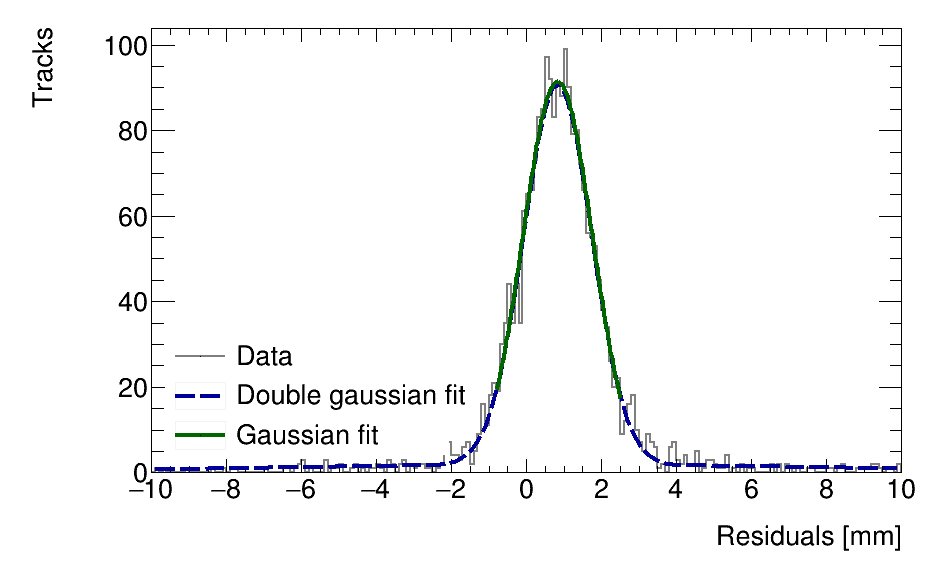
\includegraphics[width = \textwidth]{figures/figure_double_gaussian_quick_and_dirty_2900V_log_scale_gaussian_QL2C04_2900V_2021-02-08_2_xbin_10_ybin_5_100mm.png}
    \caption{Residual distribution for tracks on layer 1 built from hits on layers 3 and 4 for $x\in\left[-3.00, 97.00\right],  y\in\left[394.60, 494.60\right] mm$ fit with a double gaussian and a single gaussian in a range of $\pm$1 RMS from the histogram mean.}
    \label{fig:double_gaussian_example_fit}
\end{figure}

For all residual distributions in \SI{100}{\milli\meter} by \SI{100}{\milli\meter} bins on layer 1 built from hits on layers 3 and 4, the difference in gaussian and double gaussian means and standard deviations is shown in figure \ref{fig:double_gaussian_compare_fits}. Since the RMS of the residual means is lesser than \SI{50}{\micro\meter}, it is safe to use the Gaussian. Moreover, this is for the tracking combination with the worst extrapolation lever arm, and so the widest distribution of means; the interpolation combinations are narrower. It is expected that the gaussian standard deviation should be larger than the double gaussian standard deviation as shown because the gaussian distribution includes the effect of the noise tracks with large residuals, while the double gaussian models them separately. For this analysis, only the residual mean is of importance, so the systematic overestimate of the signal sigma by the gaussian fit can be allowed.

\begin{figure}
    \centering
    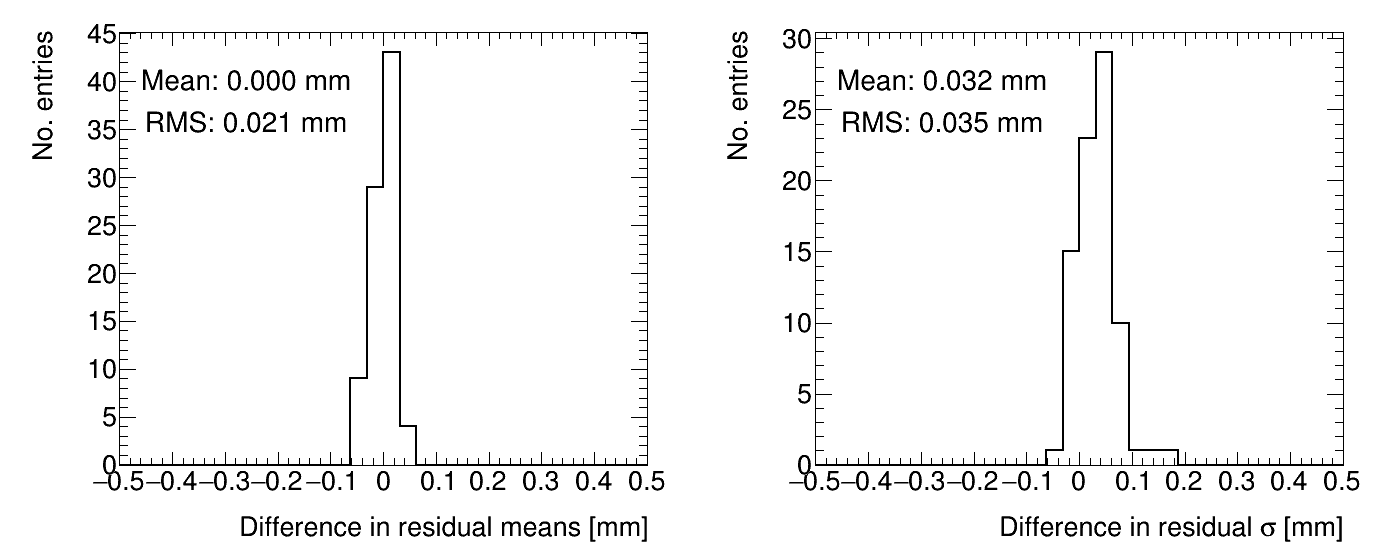
\includegraphics[width = \textwidth]{figures/figure_compare_residual_fits_QL2C04_2900V_2021-02-08_2_fit_range_mean_pm_RMS_minus_quick_and_dirty_2900V_log_scale_layer1_fixedlayers34.png}
    \caption{Difference in residual distribution means and $\sigma$'s for a gaussian and double gaussian fit.}
    \label{fig:double_gaussian_compare_fits}
\end{figure}

% --------------------------------------------------
\section{Area of residual distribution regions of interest}
% --------------------------------------------------
\label{appendix:systematics_bin_size}

% DO I NEED TO EXPLAIN THIS IN MATH? I tried on June 3rd in my notes, it's complicated for such a simple thing.
% If this flies, you'll need to establish that reference frame == two fixed layers' frame as jargon in your thesis.
% Also need to establish x == perpendicular to wires; y == perpendicular to strips. ==> How do I do this consistently?
% May need to add 3100V reference if it's not already defined in your thesis.
% Define ROI as short form?

The area of the region of interest in which to include tracks is primarily motivated by the misalignment model: the width of the region should be less than the scale on which the local offset is expected to change significantly. Changes in offset of order \SI{50}{\micro\meter} are important since this is the position resolution of the sTGCs in the $\eta$-coordinate. In a misalignment model with an offset and rotation, only the rotation changes the local offset with respect to the x-coordinate \footnote{The effect of rotation can be modeled by assuming the track position in the reference frame is related to the hit position by a passive rotation. The angle of rotation is the relative angle of the layer of interest with respect to the reference frame. The local offset does change with respect to the track's y coordinate, but negligibly in the limit of small angles.}.  The distribution of the as-built cathode board rotation angles shows that the RMS of the rotation angle is \SI{200}{\micro\radian} [https://indico.cern.ch/event/1035057/ PG. 18]; however, the distribution has a long tail, so a typical rotation angle of \SI{1000}{\micro\radian} was used here. A rotation of \SI{1000}{\micro\radian} will cause a \SI{50}{\micro\meter} change in local offset over a change in x of \SI{50}{\centi\meter}. Therefore, the width of the region of interest should be less than \SI{50}{\centi\meter}.

Two other factors also inform the width of the region. First, since the hits' x-coordinates are discrete the width in x must be larger than the pitch of the wire groups to ensure the bin will have a sufficient number of tracks fall in it. Second, more tracks will be included in a larger area so more statistics will be available for the residual distribution fit. For the bin widths wider than two wire groups, the statistics are sufficient. For each x-ray residual, the mean cosmics residual was calculated for a few different bin widths, and the difference in means plotted. Figure \ref{fig:area_bin_size_mean_diff} shows an example for QL2.C.4. The width of the distribution is on the order of \SI{50}{\micro\meter}, showing that the calculation of the residual mean is relatively robust with respect to the area of the bin. However, \SI{50}{\micro\meter} is larger than the typical statistical uncertainty on the cosmic residual of means, which ranges from \SI{10}{\micro\meter} - \SI{40}{\micro\meter} depending on the tracking combination under study. Therefore, the cosmic residual means are assigned a flat uncertainty of \SI{50}{\micro\meter}. 

\begin{figure}
    \centering
    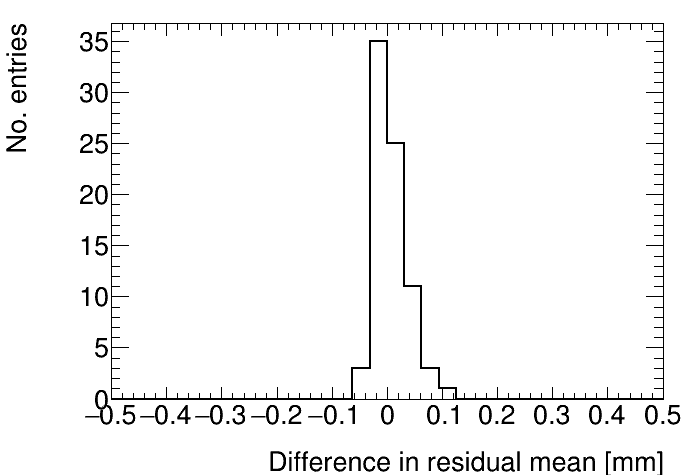
\includegraphics[width = \textwidth]{figures/compare_residual_fits_around_xrays_QL2C04_3100V_2021-05-20_100mm_width_bins_minus_QL2C04_3100V_2021-06-02_200mm_width_bins_means_difference.png}
    \caption{Difference in cosmic residual means around x-ray residuals for square bins of 100 mm width and 200 mm width for QL2.C.4.}
    \label{fig:area_bin_size_mean_diff}
\end{figure}

% --------------------------------------------------
\section{Differential non-linearity}
% --------------------------------------------------
\label{appendix:systematics_dnl}

In this context, differential non-linearity (DNL) arises from fitting the discretely sampled cluster PDO distribution, which results in shifts in the reconstructed mean depending periodically on the relative position of the avalanche with respect to the strip center, as summarized in section 2.4 of Lefebvre's thesis \cite{lefebvre_thesis} based on Endo, 1981 \cite{endo_systematic_1981}. The cluster mean can be corrected for DNL using the equation:
\begin{equation}
\label{eqn:dnl_corr}
y' = y + a \sin \left( 2 \pi y_{rel} \right)
\end{equation}

where $y$ is the cluster mean, $y_{rel}$ is the relative position of the cluster mean with respect to the strip's center, $a$ is the amplitude of the correction, and $y'$ is the corrected cluster mean. The amplitude can be derived by comparing the reconstructed hit position to the expected hit position, as done in Abusleme, 2016 \cite{abusleme_performance_2016}. With cosmic muons, there is no reference hit position to compare to, so track residuals can be used as a proxy. Lefebvre calculates the amplitude using cosmics data for sTGC quadruplets in his thesis, \cite{lefebvre_thesis} in an iterative procedure that also corrects for inter-layer misalignment. The amplitude of the corrections is ~\SI{50}{\micro\meter} for each layer and cluster size. 

\begin{figure}
    \centering
    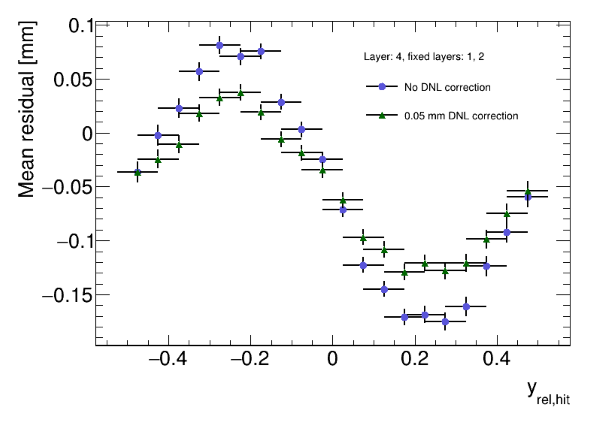
\includegraphics[width = \textwidth]{figures/figure_dnl_profiles_blue_QL2P08_3100V_2021-06-18_no_dnl_green_QL2P08_3100V_2021-06-18_2_50um_universal_DNL_layer4_fixed12.png}
    \caption{Effect applying a \SI{50}{\micro\meter} DNL correction to the cluster means on the residual vs $y_{rel}$ distribution for tracks built from layers 1 and 2 and extrapolated to layer 4 for QL2.P.8.}
    \label{fig:dnl_corr_effect}
\end{figure}

The hallmark of DNL effect is the period pattern in the $y_{rel}$ distribution, and the effect of correcting the cluster means using an amplitude of \SI{50}{\micro\meter} is shown in figure \ref{fig:dnl_corr_effect}. Although the correction is not large enough in this case, the figure shows that the correction does reduce the DNL effect. Slightly better performance is seen in the interpolation tracking combinations where the quality of the residuals is better.  

DNL corrections for cosmic muon data are difficult because the DNL effect is combined with the effect of inter-layer misalignments, shifts in the strip pattern on each board and noise. The issue is heightened in this analysis because tracks are built from two layers, and so are less robust. Moreover, the effect of the DNL correction on the mean of the residual distribution in \SI{100}{\milli\meter} by \SI{100}{\milli\meter} area is on the micrometer level in the worst extrapolation case (see \ref{fig:dnl_compare_fits}).

\begin{figure}
    \centering
    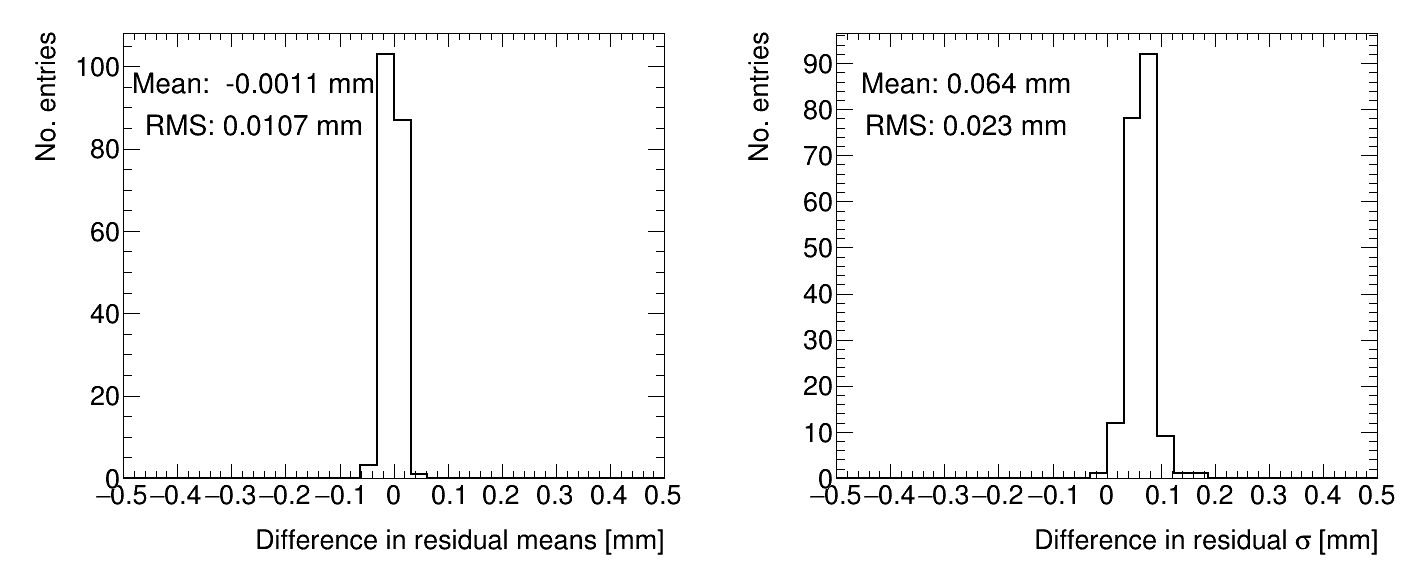
\includegraphics[width = \textwidth]{figures/figure_compare_residual_fits_QL2P08_3100V_2021-06-18_no_dnl_minus_QL2P08_3100V_2021-06-18_2_50um_universal_DNL_layer4_fixedlayers12.png}
    \caption{Difference in residual distribution means and $\sigma$'s with and without DNL correction for residuals on layer 4 from reference layers 1 and 2 for QL2.P.8.}
    \label{fig:dnl_compare_fits}
\end{figure}

The $\sigma$'s of the residual distributions do shrink with the DNL correction but not so much to affect the residual means, which are the important parameter for this analysis. Therefore, since the effect of the DNL correction is negligible, it was not pursued further.































